\chapter{Evaluation}
In order to evaluate the data and reach certain conclusions from the results it is neccessary to take a view at the data directly or atleast to visualize them in a plot or graph. For this purpose DNA offers sophisticated plotting mechanisms, automatic LaTeX output, which includes data tables and plots, and a graphical user interface namely the DNA-Visualizer.

\section{Aggregation}
The aggregation process is enabled by default and takes place at the end of the generation process. During aggregation the data from all runs will be aggregated and stored in a separate aggregation directory \textit{../aggr/} next to the run directories. The aggregations filesystem structure is analogous to the structure of a single run. The only difference is the extended data representation. All values contain the aggregated \textit{average}, \textit{minimum}, \textit{maximum}, \textit{median}, \textit{variance}, \textit{variance\textunderscore low}, \textit{variance\textunderscore up}, \textit{confidence\textunderscore low} and \textit{confidence\textunderscore up} in this order. A simple example follows:

A series is generated with 2 runs and 100 batches. The metric-value \textit{degreeMax} has the its values shown in table \ref{tab:degreemax-data} and its aggregated data in table \ref{tab:degreemax-aggr} respectively.

\begin{table}[h]
\centering
\begin{tabular}[h]{|l|l|l|}\hline
	\textbf{degreeMax} & &\\
	\hline
	\textbf{batch} & \textbf{run.0} & \textbf{run.1}\\
	\hline
	0 & 13 & 15\\
	\hline
	1 & 12 & 16\\
	\hline
	2 & 12 & 15\\
	\hline
	... & ... & ... \\
	\hline
\end{tabular}
\caption{Data values of \textit{degreeMax}.}
\label{tab:degreemax-data}
\end{table}
\begin{table}[h]
\centering
\begin{tabular}[h]{|l|l|l|l|l|l|l|l|l|l|}\hline
	\textbf{batch} & \textbf{avg} & \textbf{min} & \textbf{max} & \textbf{med} & \textbf{var} & \textbf{var-} & \textbf{var+} & \textbf{conf-} & \textbf{conf+}\\
	\hline
	0 & 14.0 & 13.0 & 15.0 & 15.0 & 1.0 & 1.0 & 1.0 & 5.013 & 22.987\\
	\hline
	1 & 14.0 & 12.0 & 16.0 & 16.0 & 4.0 & 4.0 & 4.0 & -3.975 & 31.975\\
	\hline
	2 & 13.5 & 12.0 & 15.0 & 15.0 & 2.25 & 2.25 & 2.25 & 0.019 & 26.981\\
	\hline
	... & ... & ... & ... & ... & ... & ... & ... & ... & ...\\
	\hline
\end{tabular}
\caption{Aggregated values of \textit{degreeMax}.}
\label{tab:degreemax-aggr}
\end{table}

\subsection{Configuration}
The dynamic nature of generation may cause different runs of the same series to contain different amounts of batches. This leads to the question how aggregation may handle unavailable values due to differing amounts of batches. Essentially there are two ways to approach this problem, either ignore the absent values at all or assume a specific value for them. The following sections show how one may change which approach will be used and how this affects the results using a simple example of 3 runs each with different ammount of batches.

\subsubsection{Ignore unavailable values (/n-mode)}
This is the default mode. The aggregation will completely ignore any unavailable values:
\begin{table}[h]
\centering
\begin{tabular}[h]{|l|l|l|l||l|}\hline
	\textbf{degreeMax} & & & &\\
	\hline
	\textbf{batch} & \textbf{run.1} & \textbf{run.2} & \textbf{run.3} & \textbf{average}\\
	\hline
	32 & 10 & 12 & 14 & \textbf{12}\\
	\hline
	33 & 11 & - & 17 & \textbf{14}\\
	\hline
	34 & 12 & - & - & \textbf{12}\\
	\hline
\end{tabular}
\caption{Aggregation for runs with different amount of batches in /n-mode.}
\label{tab:nmode}
\end{table}

\subsubsection{Assume unavailable values (/n+1-mode)}
The second way to handle absent values is to assume their values to be zero. This mode can be enabled on demand with:
\begin{lstlisting}
			Config.overwrite("AGGREGHATION_IGNORE_MISSING_VALUES", "false");
\end{lstlisting}
The following table shows the differences to /n-mode.
\begin{table}[h]
\centering
\begin{tabular}[h]{|l|l|l|l||l|}\hline
	\textbf{degreeMax} & & & &\\
	\hline
	\textbf{batch} & \textbf{run.1} & \textbf{run.2} & \textbf{run.3} & \textbf{average}\\
	\hline
	32 & 10 & 12 & 14 & \textbf{12}\\
	\hline
	33 & 11 & - & 17 & \textbf{9.33}\\
	\hline
	34 & 12 & - & - & \textbf{4}\\
	\hline
\end{tabular}
\caption{Aggregation for runs with different amount of batches in /n+1-mode.}
\label{tab:nmode}
\end{table}

\section{Plotting}
The plotting mechanisms included in DNA are complex and therefore only a basic example will be shown here. For more details feel free to check the plotting instruction manual. The class \textit{dna.plot.Plotting.java} offers several public methods for plotting. They usually take an array of \textit{SeriesData} objects and a destination directory as input. When the array holds multiple \textit{SeriesData}'s they will all be compared and featured in the same plots. For each plot DNA will generate a gnuplot script in the destination directory and use this to create the respective plot. Code \ref{code:plot-example} shows how to generate and plot two series and \ref{fig:plot} shows one of the resulting plots.
\begin{figure} [h]
\begin{lstlisting}
public static void main(String[] args) throws AggregationException,
		IOException, MetricNotApplicableException,
		InterruptedException {
	String dir = "data/scenario.1/";
	
	// init and generation
	GraphGenerator gg1 = new RandomGraph(GDS.undirected, 100, 300);
	BatchGenerator bg1 = new RandomBatch(5, 0, 20, 15);
	
	GraphGenerator gg2 = new RandomGraph(GDS.undirected, 200, 400);
	BatchGenerator bg2 = new RandomBatch(10, 0, 25, 30);

	Metric[] m = new Metric[] { new DegreeDistributionR(),
			new UndirectedClusteringCoefficientU() };

	Series s1 = new Series(gg1, bg1, m, dir + "s1/", "s1");
	Series s2 = new Series(gg2, bg2, m, dir + "s2/", "s2");
	
	SeriesData sd1 = s1.generate(2, 100);
	SeriesData sd2 = s2.generate(2, 100);

	// plotting
	Plotting.plot(new SeriesData[] {sd1, sd2}, dir + "plots/");
}
\end{lstlisting}
\caption{Generating two series with the same metrics and plotting them.}
\label{code:plot-example}
\end{figure}

\begin{figure} [h]
\centering
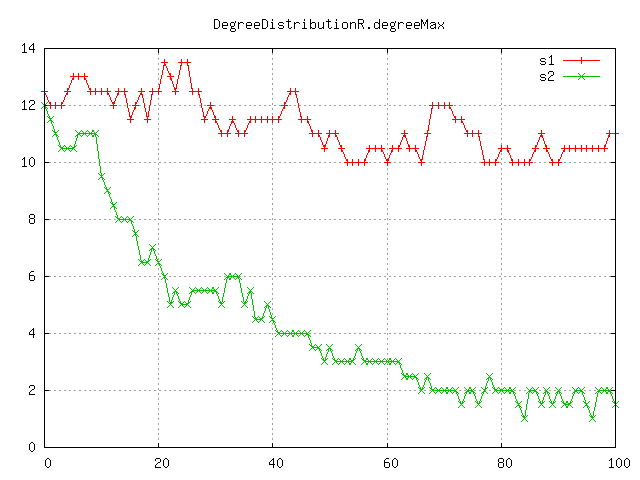
\includegraphics [scale=0.8] {images/plot}
\caption{Example plot from code snippet \ref{code:plot-example}.}
\label{fig:plot}
\end{figure}

\section{LaTeX}
The \textit{dna.latex.Latex.java} class holds several methods to generate complete latex-documents based on input series. Since the latex process itself is complex and can be configured in several ways it is recommended to check out the latex instruction manual for mor details. The code \ref{code:tex-example} shows a simple example on how to generate a series and then create a latex document including plots.
\begin{figure} [h]
\begin{lstlisting}
public static void main(String[] args) throws AggregationException,
		IOException, MetricNotApplicableException,
		InterruptedException {
	String dir = "data/scenario.1/";
	
	// init and generation
	GraphGenerator gg1 = new RandomGraph(GDS.undirected, 100, 300);
	BatchGenerator bg1 = new RandomBatch(5, 0, 20, 15);
	Metric[] m = new Metric[] { new DegreeDistributionR(),
			new UndirectedClusteringCoefficientU() };

	Series s1 = new Series(gg1, bg1, m, dir + "s1/", "s1");
	SeriesData sd1 = s1.generate(2, 100);

	// plot & generate latex document
	Latex.writeTexAndPlot(sd1, dir, "preamble.tex");
}
\end{lstlisting}
\caption{Generating series \textit{s1} and create a latex document including plots.}
\label{code:tex-example}
\end{figure}

\section{Visualization}
The DNA visualizer is a graphical user interface designed to illustrate and visualize data from single runs. A visualizer can be opened by calling the \textit{main()}-method from the \textit{dna.visualization.MainDisplay.java} class. The default configuration already allows to view all data contained in the desired run. For more instructions on how to use the visualizer and especially how to configure it check out the visualization instruction manual. See figure \ref{fig:vis} for an example.

\begin{figure} [h]
\centering
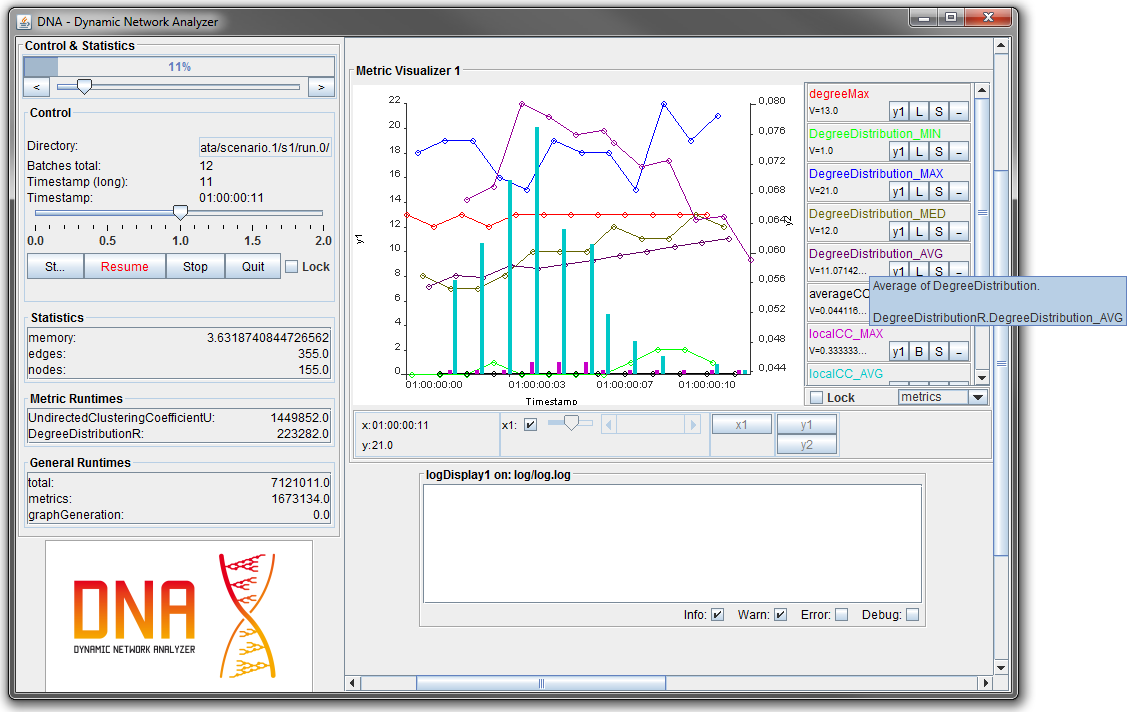
\includegraphics [scale=0.5] {images/vis-ex}
\caption{Default configured DNA visualizer.}
\label{fig:vis}
\end{figure}